\documentclass[12pt, a4paper]{article}

\renewcommand*\contentsname{Sadržaj}
\renewcommand{\figurename}{Slika}

\usepackage[margin=0.85in]{geometry}
\usepackage{graphicx}
\usepackage{float}
\usepackage{listings}
\usepackage{caption}
\usepackage{hyperref}
\renewcommand{\tablename}{Tabela}
\usepackage{fontspec}
\setmainfont{Times New Roman}
\usepackage{chngcntr}
\counterwithin{figure}{section}
\counterwithin{table}{section}

\usepackage{tikz}
\usetikzlibrary{shapes.geometric, arrows}
\tikzstyle{startstop} = [rectangle, rounded corners, minimum width=3cm, minimum height=1cm, text width=3cm, text centered, draw=black, fill=white!30]
\tikzstyle{io} = [trapezium, trapezium left angle=70, trapezium right angle=110, minimum width=3cm, minimum height=1cm, text width=3cm, text centered, draw=black, fill=white!30]
\tikzstyle{process} = [rectangle, minimum width=3cm, minimum height=1cm, text width=3cm, text centered, draw=black, fill=white!30]
\tikzstyle{decision} = [diamond, minimum width=3cm, minimum height=1cm, text width=3cm, text centered, draw=black, fill=white!30]
\tikzstyle{arrow} = [thick,->,>=stealth]


% DODANO:
\renewcommand\refname{Reference} % da pise reference u bibliografiji
\usepackage{amsmath} % za bolesne matematicke jednacine jer why not
\usepackage{algorithm2e} % za kucanje algoritama
\renewcommand{\algorithmcfname}{Algoritam} % umjesto 'Algorithm'
\renewcommand{\arraystretch}{1.5}
\renewcommand{\baselinestretch}{1}

\begin{document}

\begin{titlepage}
	\centering
	{\scshape Univerzitet u Sarajevu \par}
	{\scshape Elektrotehnički Fakultet \par}
	{\scshape Odsjek za Računarstvo i Informatiku \par}
	\vspace{2cm}
	{\Large\scshape Seminarski rad iz predmeta Optimizacija Resursa\par}
	\vspace{2.5cm}
	{\huge\bfseries Upotreba PSO Algoritma za Analizu Kriptovanog Teksta\par}
	\vspace{2.5cm}
	\Large Student: \par
	{\Large\itshape \textsc{Krupalija} Ehlimana, 1431/17461\par}
	\vfill
	Predmetni nastavnik:\par
	v. prof. dr. \textsc{Samim Konjicija}, dipl. ing. el.
	\vfill
	{\large Januar, 2019\par}
\end{titlepage}

\pagenumbering{gobble}

\section*{Sažetak}

U ovom radu predstavljeni su osnovni koncepti kriptografije, odnosno transformacije podataka zbog njihove zaštite, na kojima počiva i kriptoanaliza, koja ima zadatak da dekodira enkriptovane podatke bez poznavanja načina na koji su podaci transformisani. U tu svrhu korišten je PSO (\textit{Particle Swarm Optimization}) algoritam, koji vrši pomijeranje čestica (koje predstavljaju potencijalna rješenja) u problemskom prostoru do ispunjenja uslova zaustavljanja algoritma. Nakon prilagođavanja problema kriptoanalize \textit{cipher} transpozicijskih kriptografskih sistema u oblik pogodan za rješavanje ovim algoritmom, izvršena je njegova implementacija, testiranje performansi te analiza rezultata (s aspekta uspješnosti i efikasnosti).

\section*{Abstract}

In this paper, main ideas on which criptography (the transformation of data in order to increase their security) is founded are presented. Cryptanalysis is based on the same ideas, but its goal is to decode the encrypted data without any knowledge of the way in which the data has been transformed to its final form. In order to achieve this, PSO (\textit{Particle Swarm Optimization}) algorithm is used: it moves particles (potential solutions of the problem) in the problem area until one or more of the conditions for the algorithm's termination are fulfilled. The problem of cryptanalysing cipher transposition cryptography systems first needs to be changed so that it is suitable for being solved by this algorithm. Afterwards, the algorithm for solving this problem has been developed, its performances tested and, finally, an analysis of the results has been conducted (in terms of success in decoding the messages and efficiency in doing so).

\newpage

\tableofcontents

\newpage

\pagenumbering{arabic}
\setcounter{page}{1}

\section{Uvod}

\subsection{Opis problema}

Često postoji potreba da se podaci koje je potrebno poslati nekome zaštite od neovlaštenog pristupa. Postoji veliki broj \textbf{kriptografskih metoda} koje vrše transformaciju podataka prije njihovog slanja primaocu, kako bi se potencijalno presretanje poruke učinilo beskorisnim, odnosno kako bi se onemogućilo da osoba koja ne treba da primi poruku, ukoliko je uspije presresti, istu bude u stanju pročitati (odnosno dešifrovati). Sve ove metode mogu se podijeliti u dvije velike klase:

\begin{enumerate}

\item Metode koje koriste tajni ključ (\textbf{simetrična kriptografija}), u koje spadaju algoritmi poput \textit{Cezarovog koda};
\item Metode koje koriste javni ključ (\textbf{asimetrična kriptografija}), u koje spadaju kriptosistemi poput \textit{RSA}.

\end{enumerate}

Glavna razlika između ove dvije klase je u samom ključu, odnosno funkciji koja se koristi za transformaciju podataka (tj. njihovo skrivanje - enkripciju). Metode koje koriste tajni ključ oslanjaju se na činjenicu da bi za dešifrovanje poruke bez poznavanja ključa bilo potrebno provjeriti \textbf{veoma veliki broj kombinacija} kako bi se otkrio šablon (odnosno funkcija) kojim se može izvršiti dešifrovanje, te da takvo nešto nije izvodivo u realnom vremenu. S druge strane, metode koje koriste javni ključ ne oslanjaju se na tajnost ključa, već na \textbf{kompleksnost izračuna vrijednosti privatnih ključeva}, na osnovu kojih je dobivena vrijednost jvnih ključeva. Na ovaj način uklanja se jedan veliki sigurnosni propust metoda simetrične kriptografije: potreba za slanjem informacije o funkciji koja se koristi za enkripciju, koja se može presresti i na taj način omogućiti dekripciju originalnih podataka. \cite{cryptography} \\

Analiza enkriptovanog teksta te pokušaj rekonstrukcije funkcije za dekripciju istog problem je kojim se bavi \textbf{kriptoanaliza}. No, osim javnosti ključa i težine pronalaska pravila kojim je moguće obuhvatiti sve ulazne podatke, u analizi šifrovanih podataka potrebno je obratiti pažnju na još jednu mogućnost: da se pravilo enkripcije ne vrši nad pojedinim znakovima, već nad riječima ili blokovima podataka. Iz tog razloga, kriptografski sistemi dijele se u dvije kategorije \cite{manual}:

\begin{enumerate}

\item \textbf{Šifre} (\textit{ciphers}), pri čemu se enkripcija vrši nad pojedinim karakterima (zamjena drugim karakterima, promjena pozicije u poruci i sl.);
\item \textbf{Kodovi} (\textit{codes}), pri čemu se enkripcija vrši nad više karaktera (podaci se dijele u blokove koristeći neko pravilo, te se oni zatim tretiraju kao pojedinačni karakteri).

\end{enumerate}

\textit{Cipher} sistemi najčešće koriste vrlo jednostavne funkcije za transformaciju podataka, a te funkcije se zasnivaju ili na principu \textbf{transpozicije} (zamjene mjesta karaktera u poruci), ili na principu \textbf{substitucije} (zamjene karaktera drugim karakterima). \cite{manual} Vršenje kriptoanalize ovakvih sistema veoma je jednostavno, jer ukoliko se enkripcija vrši nad pojedinačnim karakterima, frekvencija njihovog pojavljivanja biti će jednaka frekvenciji pojavljivanja odgovarajućim karakterima jezika na kojem je poruka poslana. Na taj način moguće je veoma brzo otkriti ključ prema kojem se vrši transpozicija (ili substitucija), zbog čega se ovakvi sistemi danas najčešće ne koriste. \cite{thesis} \\

\textit{Code} sisteme mnogo je teže dekriptovati, budući da isti broj karaktera u šifrovanoj poruci mogže imati različit broj karaktera u riječi koja opisuje taj blok. I sami blokovi u okviru šifrovane poruke mogu imati varijabilnu dužinu, no u tom slučaju kompleksnost izračuna se drastično povećava, kao i narušenost sigurnosti zbog potrebe za slanjem ključa. Iz tog razloga varijabilna dužina se rijetko koristi u kodnim sistemima. \cite{manual} \\

Veliki broj različitih pristupa primjenjen je kako bi se kreirali jedinstveni algoritmi za enkripciju podataka. Rotori, \textit{shift} registri, \textit{hash} funkcije, te veliki broj protokola (poput \textit{Diffie-Hellman}-a) samo su neki od najpoznatijih. Zbog širine oblasti, u ovom radu biti će implementirano rješenje samo za transpozicijske \textit{cipher} sisteme. 

\subsection{Pregled literature}

Primarna literatura na osnovu koje je obrađen problem kriptoanalize, te algoritam \textit{Particle Swarm Optimization} koji će se koristiti za rješavanje problema, sastoji se iz sljedećih stručnih knjiga:

\begin{enumerate}

\item \textit{Basic Cryptanalysis}, priručnik za kriptoanalizu sastavljen od strane američke vojske, u kojem su objašnjeni osnovni kriptografski principi, te u kojem je moguće naći praktične primjere kriptoanalize; \cite{manual}

\item \textit{Applied Cryptanalysis: Breaking Ciphers in the Real World}, knjiga u kojoj se nalaze detaljni opisi velikog broja postojećih kriptografskih sistema te način vršenja dekripcije poruka kodiranih korištenjem istih; \cite{cryptanalysis}

\item \textit{Particle Swarm Optimization and Intelligence: Advances and Applications}, knjiga koja detaljno opisuje način rada osnovnog PSO algoritma i njegovih brojnih modifikacija; \cite{pso}

\item \textit{Particle Swarm Optimization}, knjiga u kojoj se nalaze detaljni opisi razloga, načina poboljšavanja osnovnog PSO algoritma te njihovih performansi; \cite{pso2}

\item \textit{Cryptanalysis of Block Ciphers via Improvised Particle Swarm Optimization and Extended Simulated Annealing Techniques}, članak koji opisuje pretvaranje kriptoanalitičkih problema u oblik pogodan za optimizaciju korištenjem PSO algoritma, uključujući formiranje funkcije cilja te primjenu PSO algoritma za optimizaciju iste. \cite{cryptopso}

\end{enumerate}

\subsection{Moguće aplikacije u praksi}

Kriptografija je oblast koja ima široku primjenu u praksi, jer je sigurnost neizostavan aspekt koji ni u jednom trenutku ne smije biti narušen. Kriptoanaliza je imala veliku primjenu tokom svjetskih ratova, kada je bilo neophodno presretati i dešifrovati neprijateljske poruke (koje su bile kodirane, upravo kako bi se to spriječilo), te se i danas \textbf{aktivno izučava u vojsci}. Osim mogućnosti dešifrovanja neprijateljskih poruka, kriptoanaliza je koristan alat i za poboljšavanje vlastitih kriptografskih sistema, te američka vojska koristi ovakav pristup kako bi konstantno vršila unaprjeđenje šifrovanja poruka putem traženja rješenja koje bi iste dešifrovalo. \cite{manual} \\

Kriptoanaliza ima široku primjenu i u \textbf{oblasti računarskih mreža}, gdje se koristi kako bi se testirala sigurnost \textit{hash} protokola koji se koriste kako bi se zaštitili podaci korisnika koji koriste Internet. Funkcije koje su se dugo vremena smatrale sigurnim (poput MD5 funkcije) lako su dešifrovane koristeći kriptoanalizu, te je ova nauka omogućila pronalazak slabosti takvih funkcija kako bi se iste mogle poboljšati, a samim tim i sigurnost svih korisnika. \cite{thesis2} Kriptoanaliza je oblast koja se razvija, jer se svakodnevno pronalaze novi načini za vršenje enkripcije podataka, te se u skladu s tim konstantno razvijaju i novi načini za dekripciju istih.

\newpage

\section{Korišteni Algoritam}

\subsection{Opis rada korištenog algoritma}

Algoritam koji će biti korišten za rješavanje problema kriptoanalize naziva se \textbf{\textit{Particle Swarm Optimization}}, te je napravljen po uzoru na ponašanje jata ptica i drugih grupa životinja. Ovaj algoritam pripada klasi populacijskih algoritama, odnosno u svakoj iteraciji postoji populacija - \textit{swarm} potencijalnih rješenja koja se zatim poboljšavaju dok se ne ispuni neki od uslova zaustavljanja algoritma. \cite{pso}\\

Populacija se definiše kao set od \texttt{n} čestica: \texttt{S = \{x$_1$, x$_2$, ..., x$_n$\}}, pri čemu svaka čestica predstavlja vektor od \texttt{m} elemenata: \texttt{x$_i$ = \{x$_{i1}$, x$_{i2}$, ..., x$_{im}$\}, i = 1, ..., n}.\\

Za svaku česticu računa se vrijednost funkcije cilja: \texttt{f$_i$ = f(x$_i$)}, čiji optimum je potrebno naći.\\

Za razliku od genetičkih algoritama, u kojem se stvaraju generacije populacija te vrši uništavanje čestica i njihove zamjene novim česticama, u PSO algoritmu vrši se \textbf{pomijeranje} čestica u problemskom prostoru. U tu svrhu definiše se \textbf{brzina čestice}: \texttt{v$_i$ = \{v$_{i1}$, v$_{i2}$, ..., v$_{im}$\}$^T$, i = 1, ..., n} koja omogućava da potencijalna rješenja izađu iz lokalnih ekstrema, kako bi se na taj način nastavilo pretraživanje prostora i pronalazak globalnog optimuma. \cite{pso} \\

Poput tabu pretraživanja, i u PSO algoritmu postoji mogućnost da potencijalna rješenja dođu do globalnog optimuma te zatim nastave pretraživanje prostora i pređu u nepovoljnije tačke. Iz tog razloga potrebno je imati i memoriju najboljih rješenja: \texttt{P = \{p$_1$, p$_2$, ..., p$_n$\}}, koja se sastoji od svih najboljih rješenja pojedinačnih čestica. \\

Svaka čestica ima svoje informante, odnosno čestice na osnovu čijih informacija se odlučuje u kojem smjeru će se čestica kretati. U svakoj iteraciji algoritma vrši se nasumični odabir \texttt{K} čestica koje postaju informanti čestice koja se trenutno razmatra. Zatim se čestica pomijera u onom smjeru u kojem se nalazi čestica koja ima najbolju poziciju (najbolje potencijalno rješenje). \\

U okviru algoritma vrše se dvije elementarne operacije \cite{pso}:

\begin{enumerate}

\item \textbf{Promjena brzine svih pojedinačnih čestica}, koja se računa prema sljedećoj formuli:

\begin{equation}
v_{ij}(t + 1) = c_1 \cdot v_{ij}(t) + c_2 \cdot (p_{ij}(t) - x_{ij}(t)) + c_3 \cdot (p_{gj}(t) - x_{ij}(t))
\end{equation}

\begin{equation*}
i = 1, ..., n, j = 1, ..., m
\end{equation*}

\texttt{c$_1$}, \texttt{c$_2$} i \texttt{c$_3$} predstavljaju tzv. \textbf{težinske faktore}. \texttt{p$_{ij}$} predstavlja najbolje memorisano rješenje od strane date čestice, dok \texttt{p$_{gj}$} predstavlja najbolje trenutno rješenje informanata čestice.

\item \textbf{Pomijeranje svih varijabli u problemskom prostoru}, koje se vrši prema sljedećoj formuli:

\begin{equation}
x_{ij}(t + 1) = x_{ij}(t) + v_{ij}(t + 1)
\end{equation}

\begin{equation*}
i = 1, ..., n, j = 1, ..., m
\end{equation*}

\end{enumerate}

Preporučene vrijednosti svih prethodno navedenih parametara prikazane su u Tabeli \ref{parameters}: \cite{samke}

~\\

\begin{table}[H]
\centering
\begin{tabular}{| p{4cm} | p{5cm} |}
\hline
\textbf{Parametar}		& \textbf{Preporučena vrijednost} 			\\ \hline
m 						& 20 - 40								\\ \hline
K						& 3 - 5									\\ \hline
c$_1$					& 0.7 ili 0.8								\\ \hline
c$_2$, c$_3$			& \texttt{random(0, c$_{max}$)}			\\ \hline
c$_{max}$				& 1.47 ili 1.62							\\ \hline
\end{tabular}
\caption{Preporučene vrijednosti parametara PSO algoritma}
\label{parameters}
\end{table}

~\\

Algoritam \ref{pseudocode} i Slika \ref{diagram} prikazuju pseudokod osnovne verzije PSO i način na koji on funkcioniše. Nakon inicijalizacije roja čestica i njihovih najboljih vrijednosti, iterativno se vrši izbor informanata za sve pojedinačne čestice, ažuriranje brzina svih čestica, njihovih pozicija te izračunavanje novih rješenja za sve pojedinačne čestice. Nakon toga provjerava se da li je ispunjen neki od uslova za zaustavljanje algoritma, u kojem slučaju se kao najbolje uzima najbolje od svih najboljih rješenja pojedinačnih čestica koji se nalaze u memoriji.

~\\

\begin{figure}[H]
  \centering
  \fbox{
  \begin{minipage}{.7\linewidth}
\begin{algorithm}[H]
	\textsc{PSO}(N, n, K)\\
	$t \gets $ \textsc{0}\\
	$S \gets $ \textsc{InitializeSwarm}(K, n)\\
	$P \gets $ \textsc{argmin(S)}\\
	\While{t < N} {
		\textsc{S.chooseInformants()}\\
		\textsc{S.calculateVelocities()}\\
		\textsc{S.moveParticles()}\\
		\textsc{P.updateValues(S)}\\
	}
	$\textbf{return } \textsc{min(P)}$
	\hfill \break 

 \caption{Pseudokod PSO algoritma}
 \label{pseudocode}
\end{algorithm}
  \end{minipage}
  }
\end{figure}

\begin{figure}[H]
\centering

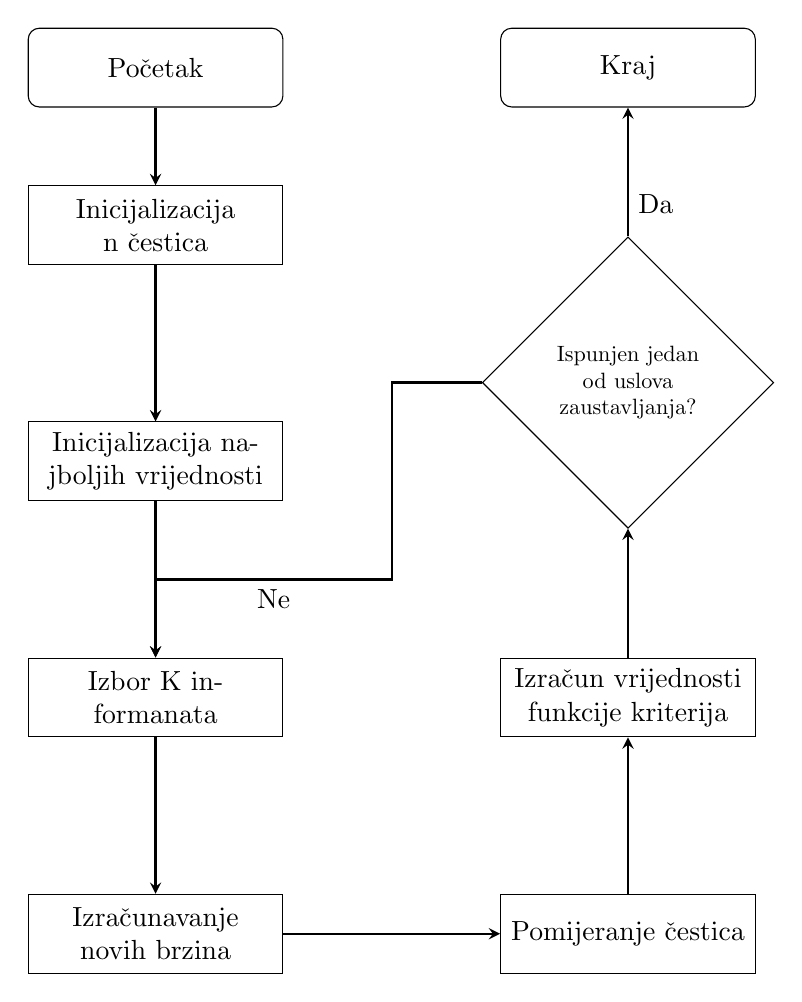
\begin{tikzpicture}[node distance = 2cm]
\node (start) [startstop] {Početak};
\node (pro1) [process, below of = start] {Inicijalizacija n čestica};
\node (pro2) [process, below of = pro1, yshift = -1 cm] {Inicijalizacija najboljih vrijednosti};
\node (pro3) [process, below of = pro2, yshift = -1 cm] {Izbor K informanata};
\node (pro4) [process, below of = pro3, yshift = -1 cm] {Izračunavanje novih brzina};
\node (pro5) [process, right of = pro4,  xshift = 4 cm] {Pomijeranje čestica};
\node (pro6) [process, right of = pro3,  xshift = 4 cm] {Izračun vrijednosti funkcije kriterija};
\node (dec) [decision, right of = pro2, xshift = 4 cm, yshift = 1 cm, text width = 3 cm, scale = 0.8] {Ispunjen jedan od uslova zaustavljanja?};
\node (stop) [startstop, right of = start, xshift = 4 cm] {Kraj};
\draw [arrow] (start) -- (pro1);
\draw [arrow] (pro1) -- (pro2);
\draw [arrow] (pro2) -- (pro3);
\draw [arrow] (pro3) -- (pro4);
\draw [arrow] (pro4) -- (pro5);
\draw [arrow] (pro5) -- (pro6);
\draw [arrow] (pro6) -- (dec);
\draw [arrow] (dec) -- ++(-3,0) -- ++(0,-2.5) -|  node[anchor = west, below, pos = 0.25]{Ne} (pro3);
\draw [arrow] (dec) -- node[anchor = north, right, pos = 0.25] {Da} (stop);
\end{tikzpicture}

\caption{Blok-dijagram PSO algoritma}
\label{diagram}
\end{figure}

Postoji mnogo načina da se izvrši poboljšanje osnovnog algoritma, a neki od njjih su: \cite{pso}

\begin{enumerate}

\item \textbf{Uvođenje inercijske težine}: \\

Brzina je veličina koja direktno utječe na promjenu pozicije svih čestica, odnosno na pomijeranje potencijalnih rješenja u problemskom prostoru. Osnovna formula za promjenu brzine pokazala se neadekvatnom, zbog pojave tzv. \textbf{\textit{swarm explosion}} efekta, pri čemu se brzina za veoma kratko vrijeme dostigne tako velike vrijednosti da sve čestice divergiraju, te je za posljedicu pronalazak najboljeg rješenja teško moguće (budući da se čestice ne teže k pretraživanju prostora koji nudi bolja potencijalna rješenja). \\

Prvi pokušaj da se riješi problem divergencije čestica bio je uvođenje maksimalne brzine, no u tom slučaju, iako nema potpune divergencije čestica, nema ni njihove konvergencije k najboljem rješenju. Umjesto da se koncentrišu u okolini najboljih rješenja, čestice napuštaju taj dio problemskog prostora i osciliraju oko ekstrema, bez mogućnosti da ga pronađu. \cite{pso} \\ 

Iz ovog razloga uvedena je nova veličina koja se naziva \textbf{inercijskom težinom}, čija je funkcija stabilizacija brzine, odnosno smanjenje perturbacija koje dovode do oscilacije čestica od povoljnih potencijalnih rješenja. Inercijska težina \texttt{w} mijenja vrijednost prethodne brzine, kako bi ona imala što manji utjecaj na njenu novu vrijednost, prema sljedećoj formuli: \cite{pso}

\begin{equation}
v_{ij}(t + 1) = w \cdot c_1 \cdot v_{ij}(t) + c_2 \cdot (p_{ij}(t) - x_{ij}(t)) + c_3 \cdot (p_{gj}(t) - x_{ij}(t))
\end{equation}

\begin{equation*}
i = 1, ..., n, j = 1, ..., m
\end{equation*}

\item \textbf{Uvođenje susjedstva}: \\

U osnovnoj verziji PSO algoritma, sve čestice imaju memoriju u kojoj se nalazi najpovoljnija tačka koja je posjećena do datog trenutka. To znači da je za memoriju potrebno izdvojiti istu količinu resursa kao i za same čestice, odnosno da za \texttt{m} čestica treba postojati i \texttt{m} varijabli koje čuvaju informaciju o najboljim rješenjima. \\

Kako bi se smanjila količina resursa potrebnih za čuvanje informacija o najboljim rješenjima, uveden je koncept \textbf{susjedstva}, koji se zasniva na udaljenosti čestica jednih od drugih, no ne u prostornom smislu (bez obzira na moguću razliku u prostornoj udaljenosti, susjedima se smatraju one čestice koje su najbliže jedne drugima, što se naziva socijalnim susjedstvom, u odnosu na klasično geografsko susjedstvo). Za \texttt{k} susjeda formira se ciklus koji povezuje jednu memorijsku ćeliju sa svim odabranim susjedima. Ažuriranje memorije se vrši samo ukoliko se pronađe rješenje koje je bolje od najboljeg dotad pronađenog rješenja (od svih susjednih čestica). Na ovaj način štede se resursi, smanjuje se broj upisa u memoriju, te broj neophodnih poređenja svih ćelija memorije na kraju rada programa. \cite{pso2}

\item \textbf{Uvođenje većeg broja \textit{swarm}-ova}: \\

Kako bi pretraživanje prostora bilo još efikasnije, odnosno kako bi se u što kraćem vremenu pretražio što veći prostor, uvedena je modifikacija PSO algoritma koja se naziva \textbf{grupni PSO}. U okviru ovog algoritma kreira se više \textit{swarm}-ova, pri čemu su svi neovisni jedni o drugima i imaju vlastite funkcije za pomijeranje i brzinu. \\

U idealnom slučaju, svi \textit{swarm}-ovi nalaze se u različitim dijelovima problemskog prostora, te čuvaju informacije o svojim globalnim ekstremima, od kojih se na kraju rada programa bira najbolji. Iako je preklapanje nekih čestica veoma teško izbjeći (posebno u slučaju kada se koristi veliki broj \textit{swarm}-ova), ova modifikacija pokazala se kao nešto brža u odnosu na osnovnu verziju PSO algoritma. Budući da je pogodan i za paralelno izvršavanje, grupni PSO može postići još bolje performanse ukoliko se različiti dijelovi algoritma (pretraživanje problemskog prostora koristeći različite \textit{swarm}-ove) budu izvršavali u isto vrijeme. \cite{cryptopso}

\end{enumerate}

\subsection{Svođenje opisanog problema u formu korištenog algoritma}

PSO je algoritam koji vrši traženje optimuma date funkcije cilja. U problemu kriptoanalize potrebno je izvršiti dekodiranje enkriptovane poruke sa što manje grešaka, te iz tog razloga cilj optimizacije predstavlja \textbf{tačnost dekodirane poruke}, odnosno što manje odstupanje dekodirane poruke od prirodnog jezika. \\

\textbf{Potencijalna rješenja} predstavljaju vrijednosti dekodiranih poruka, odnosno permutacije karaktera engleskog jezika koje se sastoje od predefinisanog broja karaktera. Budući da je i za relativno mali broj karaktera broj njihovih permutacija veoma veliki (\texttt{n!}), problemski prostor u kojem se vrši pretraživanje biti će veoma veliki, te će se na ovaj način moći izvršiti adekvatno testiranje PSO algoritma pri rješavanju problema kriptoanalize. \\

\textbf{Funkcija kriterija} je sličnost frekvencija karaktera u poruci predefinisanim frekvencijama karaktera engleskog jezika. Što je veća sličnost, to je veća mogućnost da potencijalno rješenje ima smisla (odnosno, da predstavlja neku smislenu poruku), s tim da bi vrijednost funkcije kriterija bila ista za sve permutacije dekodirane poruke (od kojih je samo jedna tačna), te se iz tog razloga u funkciju kriterija uvodi i sličnost frekvencija parova karaktera \cite{cryptopso} (kako bi bolju vrijednost imala npr. permutacija \texttt{SENDHELP} od \texttt{ENDESHLP}, bez obzira što su frekvencije karaktera u oba slučaja iste). \\

Frekvencije pojedinačnih karaktera (\textit{monograma}), kombinacija od po dva karaktera (\textit{bigrama}), kombinacija od po tri karaktera (\textit{trigrama}) i kombinacija od po četiri karaktera (\textit{quadgrama}) engleskog jezika koje će biti korištene pri kriptoanalizi izračunate su na osnovu analize teksta koji se sastoji od nekoliko milijardi karaktera, iz kojeg razloga imaju dovoljnu vjerodostojnost da bi se koristile u analizi poruka. \cite{letters}

Postoje tri funkcije kriterija, koje se koriste u različitim dijelovima algoritma:

\begin{enumerate}

\item \textit{Bigram} funkcija, koja vrši usporedbu da li se \textit{bigrami} u poruci razlikuju od standardne frekvencije \textit{bigrama}:

\begin{equation}
f(x) = \sum_{i = 1}^{26}{\sum_{j = 1}^{26}{SDF[i, j] - DDF[i, j]}}
\end{equation}

\item \textit{Trigram} funkcija, koja vrši usporedbu da li se \textit{trigrami} u poruci razlikuju od standardne frekvencije \textit{trigrama}:

\begin{equation}
f(x) = \sum_{i = 1}^{26}{\sum_{j = 1}^{26}{\sum_{k = 1}^{26}{STF[i, j, k] - DTF[i, j, k]}}}
\end{equation}

\item \textit{Quadgram} funkcija, koja vrši usporedbu da li se \textit{quadgrami} u poruci razlikuju od standardne frekvencije \textit{quadgrama}:

\begin{equation}
f(x) = \sum_{i = 1}^{26}{\sum_{j = 1}^{26}{\sum_{k = 1}^{26}{\sum_{l = 1}^{26}{SQF[i, j, k, l] - DQF[i, j, k, l]}}}}
\end{equation}

\end{enumerate}

Veličine u funkcijama kriterija imaju sljedeća značenja:

\begin{itemize}
\renewcommand\labelitemi{--}

\item \texttt{SDF[i, j]}: standardna frekvencija \textit{bigrama} (niza od dva karaktera) koja se izračunava na osnovu podataka iz \cite{letters};
\item \texttt{DDF[i, j]}: frekvencija \textit{bigrama} izmjerena u poruci \texttt{x} koja predstavlja potencijalno rješenje;
\item \texttt{STF[i, j, k]}: standardna frekvencija \textit{trigrama} (niza od tri karaktera) koja se izračunava na osnovu podataka iz \cite{letters};
\item \texttt{DTF[i, j, k]}: frekvencija \textit{trigrama} izmjerena u poruci \texttt{x} koja predstavlja potencijalno rješenje;
\item \texttt{SQF[i, j, k, l]}: standardna frekvencija \textit{quadgrama} (niza od četiri karaktera) koja se izračunava na osnovu podataka iz \cite{letters};
\item \texttt{DQF[i, j, k, l]}: frekvencija \textit{quadgrama} izmjerena u poruci \texttt{x} koja predstavlja potencijalno rješenje.

\end{itemize}

Cilj algoritma je \textbf{minimizacija} ove funkcije - optimalno rješenje je ono koje je najprirodnije, tj. ono koje najmanje odstupa od prirodnog jezika (što je ispunjeno kad su frekvencije pojedinačnih karaktera i bigrama najsličnije standardnim frekvencijama).

Algoritam ima sljedeće uslove zaustavljanja:

\begin{enumerate}

\item \textbf{Dostizanje maksimalnog broja iteracija} (parametra koji je moguće mijenjati), koji za cilj ima zaustavljanje rada algoritma nakon pomijeranja čestica dovoljan broj puta. Veličina ovog parametra određuje se testiranjem, te može varirati ovisno o problemu koji se rješava. Broj iteracija ne smije biti premali, jer u tom slučaju čestice ne istraže prostor dovoljno i ne konvergiraju ka optimumu, no broj iteracija ne smije biti ni prevelik, jer u tom slučaju vrijeme izvršavanja algoritma može postati neprihvatljivo dugo.
\item \textbf{Izlazak svih čestica iz dopuštenog prostora}, u kom slučaju više nema čestica koje generišu nova rješenja (jer su pozicije svih čestica nedozvoljene). Čestice dolaze u nedozvoljenu poziciju u trenutku kad više nema mogućnosti za poboljšavanjem rješenja, a čestice nisu dostigle optimalno rješenje (u tom slučaju, svako novo rješenje bi dostizalo gore vrijednosti, tako da se takve čestice prestaju razmatrati).
\item \textbf{Dostizanje optimalne vrijednosti}, odnosno trenutak u kojem se pronađe čestica s vrijednošću greške jednakom 0 (a samim tim i vrijednošću funkcije cilja jednakom minimalnoj vrijednosti, koja također iznosi 0).

\end{enumerate}

\textbf{Konvergencija čestica} (odnosno nepronalazak boljeg rješenja nakon jedne iteracije) ne predstavlja uslov zaustavljanja algoritma, jer se brzina čestica mijenja u ovisnosti o boljim pozicijama drugih čestica (informanata), koji se određuju nasumično. Ukoliko se u nekoliko iteracija ne pronađe nijedno bolje rješenje, brzine čestica će se promijeniti na takav način da se približavaju česticama koje imaju povoljnije pozicije, te će se nakon nekog vremena početi generisati bolje pozicije (ukoliko takve postoje). \\

\textbf{Brzine čestica} su \texttt{Boolean} vrijednosti, odnosno mogu imati vrijednost \texttt{True} (to znači da se slovo nalazi na pogrešnoj poziciji) ili \texttt{False} (to znači da slovo čini \textit{bigram, trigram ili quadgram}, u kom slučaju se ne treba kretati). \\

Postoji više vrsta pomijeranja čestica u problemskom prostoru: \\

\begin{itemize}
\renewcommand\labelitemi{--}

\item \textbf{Permutiranje karaktera} koji se ne nalaze na ispravnim pozicijama, koje se vrši na dva načina (svaki način ima 50 \% šanse odabira):

\begin{enumerate}

\item Generisanjem nasumične konfiguracije kojom će se svi neispravno pozicionirani karakteri repozicionirati na nove pozicije;

\item Pronalaskom mjesta na kojem se neki od karaktera koje je potrebno permutirati nalaze u poziciji najboljeg informanta, nakon čega se na to mjesto umeće traženi karakter.

\end{enumerate}

\item \textbf{Umetanje karaktera} između ispravno pozicioniranih blokova, što se izvršava u posebnom slučaju kada je broj neispravno pozicioniranih karaktera manji od dužine bloka, nakon čega nema mogućnosti da se prethodno opisanim mehanizmom uopće promijeni (a kamoli poboljša) vrijednost funkcije cilja;

\item \textbf{Promjena funkcije kriterija} (i svih pripadajućih funkcija za izračunavanje frekvencija blokova karaktera), nakon što ne postoje karakteri koje je potrebno permutirati, a nije dostignuta optimalna vrijednost funkcije cilja. U ovom slučaju svi karakteri čine dio nekog bloka, te ih je kao takve nemoguće modificirati koristeći bilo koji od prethodno navedenih mehanizama.

\end{itemize}

\newpage

\section{Simulacijski rezultati}

\subsection{Implementacija rješenja}

Prvi korak u implementaciji rješenja je izračunavanje prirodnih frekvencija. Neophodne frekvencije učitavaju se iz \textit{file}-ova \texttt{monograms.txt, bigrams.txt, trigrams.txt} i \texttt{quadgrams.txt} (za testne svrhe, zbog kratkoće poruka njihove frekvencije uvijek previše odstupaju od prirodnih, pa je u tom slučaju izvršeno računanje prirodne frekvencije samo za karaktere poruke). \\

Izračunavanje prirodnih frekvencija karaktera implementirano je u okviru funkcija: \texttt{natural- Monograms, naturalBigrams, naturalTrigrams} i \texttt{naturalQuadgrams}. Izračunavanje frekvencija za datu poruku implementirano je u okviru funkcije \texttt{calculateMessageFrequencies}, koja zatim poziva funkcije \texttt{findFrequenciesCharacters, findFrequenciesBigrams, findFrequen- ciesTrigrams} i \texttt{findFrequenciesQuadgrams} koje vrše pojedinačne izračune. \\

Funkcija \texttt{toString} vrši pretvaranje niza cjelobrojnih vrijednosti (što je način čuvanja koordinata rješenja) u niz karaktera, odnosno poruku. \\

Funkcija \texttt{transpozition} vrši kreiranje kodirane poruke, odnosno pravi nasumičnu konfiguraciju poruke koja se sastoji od istih karaktera, no koji se nalaze na različitim mjestima. \\

Funkcije \texttt{CaesarCode} i \texttt{CaesarDecode} vrše kodiranje i dekodiranje poruke respektivno korištenjem Cezarovog koda s nasumičnom vrijednošću ključa. \\

Funkcije kriterija, odnosno funkcije koje vrše izračun greške - odstupanja od prirodnih frekvencija su funkcije \texttt{criterionFunctionBigrams, criterionFunctionTrigrams} i \texttt{criterion \\ FunctionQuadgrams}. \\

Funkcije koje vrše ažuriranje brzine čestice ovisno o tome da li se neki karakter ili blok karaktera nalaze na ispravnoj poziciji su funkcije \texttt{findCorrectBigrams, findCorrectTrigrams} i \texttt{find- CorrectQuadgrams}. \\

Funkcije koje vrše pronalazak prvog ili neispravnog bloka karakteru sa specificiranim rednim brojem su funkcije \texttt{findIncorrectBigram, findIncorrectTrigram} i \texttt{findIncorrectQuadgram}. \\

Klasa \texttt{Particle}, osim konstruktora, posjeduje i metodu \texttt{move} koja, uz korištenje prethodno navedenih funkcija i poštivanje koncepata koji su prethodno opisani u radu, vrši pomijeranje čestice, promjenu režima rada (da li se posmatraju \textit{bigram}-i ili veći blokovi karaktera) i ažuriranje svoje brzine. \\

Klasa \texttt{SwarmOfParticles}, osim inicijalizacije, posjeduje i funkciju \texttt{moveAllParticles}, u okviru koje se vrši jedna iteracija algoritma - pomijeranje svih čestica i ažuriranje svih neophodnih parametara.

\subsection{Postavka simulacija}

Prethodno opisani algoritam implementiran je u programskom jeziku \textit{Python}. Cijela implementacija rješavanja problema kriptoanalize koristeći PSO algoritam dostupna je na: \\ \href{https://github.com/ehlymana/PSOCryptanalysis}{https://github.com/ehlymana/PSOCryptanalysis}. Izgled simulacijske aplikacije prikazan je na Slici \ref{gui}.

\begin{figure}[H]

\center
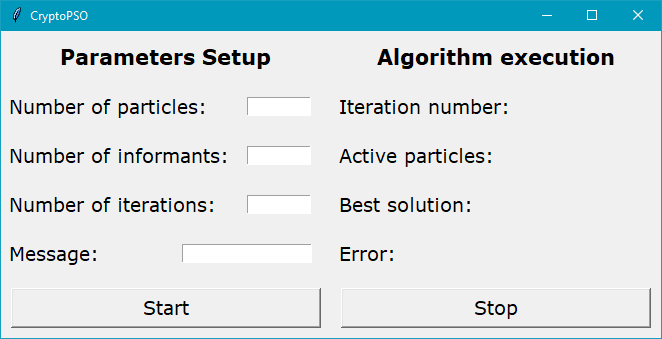
\includegraphics[scale=0.7]{res/gui.png}
\caption{Simulacijska aplikacija}
\label{gui}

\end{figure}

Aplikacija prihvata samo riječi (ili više riječi bez razmaka) koje se sastoje od velikih slova engleskog alfabeta. Nakon unošenja početnih parametara (broj čestica u roju, broj informanata i broj iteracija) i pritiska na dugme \textbf{Start}, vrši se inicijalizacija početnog roja čestica te iterativno pomijeranje čestica u problemskom prostoru. \\

Na ekranu se prikazuju rezultati izvršavanja algoritma u iterativnom postupku. Prikazuje se dekodirana trenutno najbolja poruka, vrijednost greške u odnosu na stvarnu vrijednost, kao i broj trenutno aktivnih čestica. \\

U svakom trenutku moguće je prekinuti izvršavanje algoritma pritiskom na dugme \textbf{Stop}, u kojem slučaju se najbolje rješenje iz trenutne iteracije proglašava za finalno rješenje. \\

Aplikacija je testirana na više načina, koristeći različite kriterije za performanse, koje će biti opisane u nastavku.

\subsection{Rezultati izvršavanja za različite dužine poruka}

Kako bi se dobili što relevantniji i konzistentniji rezultati, za ovu vrstu testiranja korišten je \textbf{konstantan broj} čestica (\texttt{40}), informanata (\texttt{4}) i iteracija (\texttt{50}). Taj broj odabran je u skladu s preporukama za \textbf{optimalne vrijednosti} \cite{samke}, kako bi vjerovatnoća za pronalaskom rješenja bila ista (i što veća) bez obzira na varijabilnu dužinu poruka. \\

Simulacije su za dužine znakova manje od 10 pokrenute po \texttt{10} puta, kako bi se smanjio utjecaj randomizma (koji je prisutan u ovom algoritmu) na konačne performanse. Zbog predugog trajanja izvršavanja, simulacije za dužine znakova veće od 9 pokrenute su \textbf{samo jednom}. Rezultati simulacije prikazani su u Tabeli \ref{poruke}:

\begin{itemize}
\renewcommand\labelitemi{--}

\item Sve poruke predstavljaju validne riječi, ili nizove riječi engleskog jezika;
\item Dužina poruka varira između 1 i 15 (vrijeme izvršavanja za veće dužine poruka je predugo);
\item Najbolja finalna rješenja u skladu su s vrijednošću greške, pri čemu je broj karaktera koji su pogrešno pozicionirani jednak vrijednosti greške;
\item Broj iteracija za dolazak do rješenja povećava se s povećanjem dužine poruke, zbog drastičnog povećanja broja permutacija;
\item Vrijeme izvršavanja mjereno je u sekundama, te je vidljivo njegovo drastično povećanje za veću dužinu poruka.

\end{itemize}

\begin{table}[H]
\centering
\begin{tabular}{ | l | p{1.5 cm} | l | p{2 cm} | p{1.5 cm} | p{1.5 cm} |} \hline
\textbf{Poruka} 			& \textbf{Dužina poruke}	& \textbf{Finalno rješenje}		& \textbf{Vrijednost greške} 	& \textbf{Broj iteracija}	& \textbf{Vrijeme izvršavanja}	\\ \hline
A 						& 1						& A 						& 0							& 0						& 0.338						\\ \hline
TO 						& 2						& TO 						& 0							& 0						& 0.435						\\ \hline
THE						& 3						& THE						& 0							& 0						& 0.456 						\\ \hline
STAR					& 4						& STAR						& 0							& 0						& 0.314						\\ \hline
APRIL					& 5						& APRIL						& 0							& 0						& 0.404						\\ \hline
BIRDIE					& 6						& BIRDIE					& 0							& 0.4					& 0.666						\\ \hline
SOMEDAY				& 7						& SOMEDAY					& 0							& 1.1					& 0.684						\\ \hline
COMPUTER				& 8						& COMPUTER				& 0							& 2.6					& 1.242						\\ \hline
YESTERDAY				& 9						& YESTERDAY				& 0							& 5.8					& 67.471					\\ \hline
BEPEACEFUL				& 10					& BEPEACEFUL				& 0							& 6						& 16.435					\\ \hline
SHAKESPEARE			& 11					& SHAKESPEARE 				& 0							& 8						& 21.911					\\ \hline
THEGOLDENSUN			& 12					& THEGOLDENSUN			& 0							& 9						& 48.137					\\ \hline
CONSTELLATION			& 13					& CONSTELATIONL			& 1							& 50					& 1310.583					\\ \hline
CHEYENNEANTHEM		& 14					& MYTINDIMESPENG	 		& 1							& 50					& 2394.452					\\ \hline
SEAGULLJONATHAN		& 15					& AGULLJONHANATSE 		& 2							& 50					& 3489.189					\\ \hline
\end{tabular}
\caption{Rezultati testiranja za različite dužine poruka}
\label{poruke}
\end{table}

\subsection{Rezultati izvršavanja za različite vrijednosti parametara}

U svrhu testiranja, izvršena je modifikacija sljedećih parametara:

\begin{itemize}
\renewcommand\labelitemi{--}

\item \textbf{Broj iteracija}: U ovisnosti od broja iteracija, vrijednost pronađenog rješenja trebala bi se mijenjati na način da je tačnost za veći broj iteracija veća;
\item \textbf{Broj čestica}: Za manji broj čestica, biti će generisan manji broj početnih konfiguracija, zbog čega će biti teže formirati ispravne konfiguracije (potreba za mijenjanjem \textit{quadgram}-a dovesti će do povećanja trajanja izvršavanja programa);
\item \textbf{Broj informanata}: Veći broj informanata trebao bi osigurati brže poboljšanje tačnosti rješenja, zbog veće mogućnosti da je neko od informanata (kojih ima više) u ispravnoj konfiguraciji.

\end{itemize}

Svi ostali parametri imaju standardne vrijednosti (broj čestica: \texttt{40}, broj informanata: \texttt{4}, dužina poruke: \texttt{8}, broj iteracija: \texttt{40}), kako bi njihov utjecaj na izvršavanje programa bio minimalan. Svaka simulacija pokrenuta je 10 puta, te rezultati predstavljaju srednju vrijednost rezultata tokom svih 10 pokretanja. Rezultati simulacije prikazani su u Tabelama \ref{iteracije} - \ref{informanti}:

\begin{table}[H]
\centering
\begin{tabular}{| c | c | c |} \hline
\textbf{Broj iteracija}		& \textbf{Srednja vrijednost greške}	& \textbf{Vrijeme izvršavanja}		\\ \hline
1						& 1.7								& 0.503								\\ \hline
10						& 0									& 0.668								\\ \hline
25						& 0									& 1.375								\\ \hline
50						& 0									& 0.81								\\ \hline
100						& 0									& 0.82								\\ \hline
250						& 0									& 1.677								\\ \hline
500						& 0									& 0.595								\\ \hline
1000					& 0									& 0.625								\\ \hline
\end{tabular}
\caption{Rezultati testiranja za različit broj iteracija}
\label{iteracije}
\end{table}

\begin{table}[H]
\centering
\begin{tabular}{| c | c | c |} \hline
\textbf{Broj čestica}		& \textbf{Srednja vrijednost greške}	& \textbf{Vrijeme izvršavanja}		\\ \hline
1						& 1.3								& 38.213							\\ \hline
2						& 0.6								& 103.673							\\ \hline
5						& 0.1								& 14.487							\\ \hline
10						& 0									& 0.477								\\ \hline
25						& 0									& 0.65								\\ \hline
50						& 0									& 0.666								\\ \hline
100						& 0									& 0.94								\\ \hline
125						& 0									& 0.914								\\ \hline
150						& 0									& 0.979								\\ \hline
\end{tabular}
\caption{Rezultati testiranja za različit broj čestica}
\label{cestice}
\end{table}

\begin{table}[H]
\centering
\begin{tabular}{| c | c | c |} \hline
\textbf{Broj informanata}	& \textbf{Srednja vrijednost greške}	& \textbf{Vrijeme izvršavanja}	\\ \hline
1						& 0									& 0.845							\\ \hline
2						& 0									& 0.522							\\ \hline
3						& 0									& 1.781							\\ \hline
4						& 0									& 0.613							\\ \hline
5						& 0									& 0.926							\\ \hline
10						& 0									& 1.018							\\ \hline
25						& 0									& 1.848							\\ \hline
\end{tabular}
\caption{Rezultati testiranja za različit broj informanata}
\label{informanti}
\end{table}

\subsection{Zaključci}

Nakon provedenih testiranja, mogu se lako identificirati dobre i loše strane implementirane aplikacije. Korištenje \textit{bigram}-a, \textit{trigram}-a i \textit{quadgram}-a omogućava \textbf{gotovo 100 \%-nu tačnost} pri dekodiranju poruka, no iz tog razloga vremenske performanse algoritma su \textbf{veoma loše}, pri čemu za dekodiranje poruke od 15 karaktera treba \textbf{oko 60 minuta}. \\

Iako na tačnost dekodiranja utječu parametri poput broja čestica, iteracija i informanata, njihova uloga \textbf{nije presudna}, te je praćenje preporučenih vrijednosti dovoljno (iako su i mnogo manje veličine dovoljne) kako bi se poruke ovih veličina uspješno dekodirale. Povećanje broja iteracija neko vrijeme poboljšava performanse algoritma, nakon čega one ostaju performanse (razlika između 500 i 1000 iteracija je neznatna). S druge strane, povećanje broja čestica drastično smanjuje trajanje izvršavanja, budući da se vjerovatnoća da će se neka od čestica brzo naći u tačnoj konfiguraciji povećava s brojem čestica. No, za prevelik broj čestica performanse algoritma počinju da degradiraju, zbog čega ovaj broj ne smije biti ni preveliki (posebno s aspekta memorije). Povećanje broja informanata nema nekog značajnog utjecaja na izvršavanje programa.

\newpage

\section{Zaključak}

PSO algoritam moguće je \textbf{uspješno iskoristiti} za dekodiranje šifrovanih poruka koristeći osobine prirodnih jezika (odnosno, prirodnu frekvenciju). Cezarov kod pokazao se kao \textbf{potpuno nevažan} za samo dekodiranje, jer je dovoljno pokrenuti funkciju za identifikaciju takvog kodiranja u poruci kako bi se dobili izvorni karakteri (koji su, naravno, transponirani, nakon čega kreće proces kriptoanalize koristeći prethodno opisane koncepte). No, kao ključni problem nameće se \textbf{vrijeme izvršavanja} algoritma, jer osobina PSO algoritma da se nakon nasumične incijalizacije vrijednosti čestica poboljšavaju ovisno o najboljim pronađenim \textbf{nije dovoljna} kako bi se prevazišli problemi proizvedeni kroz sam algoritam kriptoanalize. \\

Prvobitni problem predstavlja \textbf{veličina problemskog prostora}, odnosno broj permutacija karaktera koji čine poruku, koji je već za male veličine poruka izrazito veliki, što drastično smanjuje vjerovatnoću da će bilo koja od inicijalnih vrijednosti čestica posjedovati bilo kakvu karakteristiku tačnog rješenja: tačne \textit{bigram}-e, \textit{trigram}-e ili čak \textit{quadgram}-e. PSO algoritam \textbf{nije namijenjen za rješavanje ovakvih problema}, posebno iz razloga što brzina ne predstavlja broj za koji se vrijednost rješenja povećava ili smanjuje, već je prilagođena tako da predstavlja vrijednost koja pokazuje da li je traženi karakter dio ispravne konfiguracije ili ga je potrebno ponovo permutirati. Informanti također pružaju \textbf{limitirane informacije} o boljim rješenjima, jer je sama veza između različitih rješenja nejasna: na nivou \textit{bigram}-a ili drugih blokova karaktera, informanti ne mogu dati mnogo korisnih informacija, jer su i njihove informacije samo parcijalno tačne, što može dovesti do degradacije rješenja. \\

Drugi problem predstavlja \textbf{trajanje izvršavanja}, na koje uveliko utječe korištenje \textit{quadgram}-a u algoritmu, pri čemu se u svakoj iteraciji algoritma prolazi kroz četverostruku petlju (26$^4$), što drastično pogoršava performanse algoritma. No, s povećavanjem broja karaktera u poruci, korištenje manjih blokova karaktera jednostavno \textbf{nije dovoljno} da bi se dobili tačni rezultati (prevelika je vjerovatnoća da se više karaktera može naći u tako malim nizovima, te algoritam tvori pogrešne kombinacije koje imaju malu grešku s aspekta razlike u prirodnoj frekvenciji), zbog čega je ovaj koncept ugrađen u algoritam na samom početku razvoja. \\

Za male dužine poruka, ovaj algoritam je sasvim dovoljan da se izvrši \textbf{egzaktna i brza kriptoanaliza}, no za veće dužine poruka, njegove performanse drastično degradiraju, iz kojeg razloga bi se problem \textit{quadgram}-a trebao prevazići koristeći \textbf{manje matrice}, budući da je većina elemenata u blokovskoj matrici približno jednaka nuli (naprimjer, \textit{quadgram} \texttt{YYBB} se nikako ne pojavljuje u engleskom jeziku). Iz tog razloga nema potrebe za vršenjem velikog broja poređenja s takvim vrijednostima, te bi se performanse algoritma mogle značajno poboljšati ukoliko se funkcija kriterija za \textit{quadgram}-e promijeni, kao i sam način čuvanja matrice s ovim koeficijentima.

\newpage

\bibliographystyle{IEEEtran}
\bibliography{bibliography}

\end{document}